\documentclass[11pt,a4]{article}
\usepackage[a4paper,includeheadfoot,margin=2.54cm]{geometry}
\usepackage{graphicx}
\usepackage{rotating}
\usepackage{subcaption}
\usepackage{placeins}

\author{Stuart Reilly - 2258082R}
\title{Safety Critical Systems Assessed Exercise (H)}
\date{\today}

\begin{document}
\pagenumbering{roman}
\maketitle
\tableofcontents

\pagebreak
\pagenumbering{arabic}
\section{Introduction}
Climate change is an unavoidable issue for every industry.
With the increase in the likelihood of extreme weather events caused by climate change,
all industries must assess the risk to their services or products.
The rail network is an industry which many people rely on daily, and any disruption to
the service can lead to large knock-on effects for other industries.
As such, assessing and minimising the risk to the rail network caused by climate change
is vital to many industries.

\section{Risk Assessment Tool}
To design the risk assessment tool, first the possible issues caused by climate change to
the rail network much be researched.
The main issue for the rail network is possible train derailment.
In order to prevent train derailment, services are cancelled.
If the risk of train derailment could be reduced, less services would need to be
cancelled.
Following the top-down technique from fault trees, the following high level issues were 
found:
\begin{itemize}
	\item Power cut
	\item Train pushed over
	\item Errors with the tracks
	\item Materials on the tracks
\end{itemize}
Research into these issues lead to the following basic events:
\begin{itemize}
	\item Flooding
		\begin{itemize}
			\item Can wash away tracks
			\item Can wash away ballast, leading to unstable tracks
		\end{itemize}
	\item Extreme temperatures
		\begin{itemize}
			\item Heat leads to "sun kinks" where the track buckles do to
				thermal expansion
			\item Cold leads to brittle tracks
		\end{itemize}
	\item Extreme Winds
		\begin{itemize}
			\item Can blow debris on the tracks
			\item Can blow trains of the tracks
		\end{itemize}
	\item Landslips
		\begin{itemize}
			\item Can "wash away" tracks
		\end{itemize}
\end{itemize}

These high level events and basic events were then combined into the fault tree in
Figure \ref{fig:tool}

\begin{figure}[h]
	\begin{sideways}
		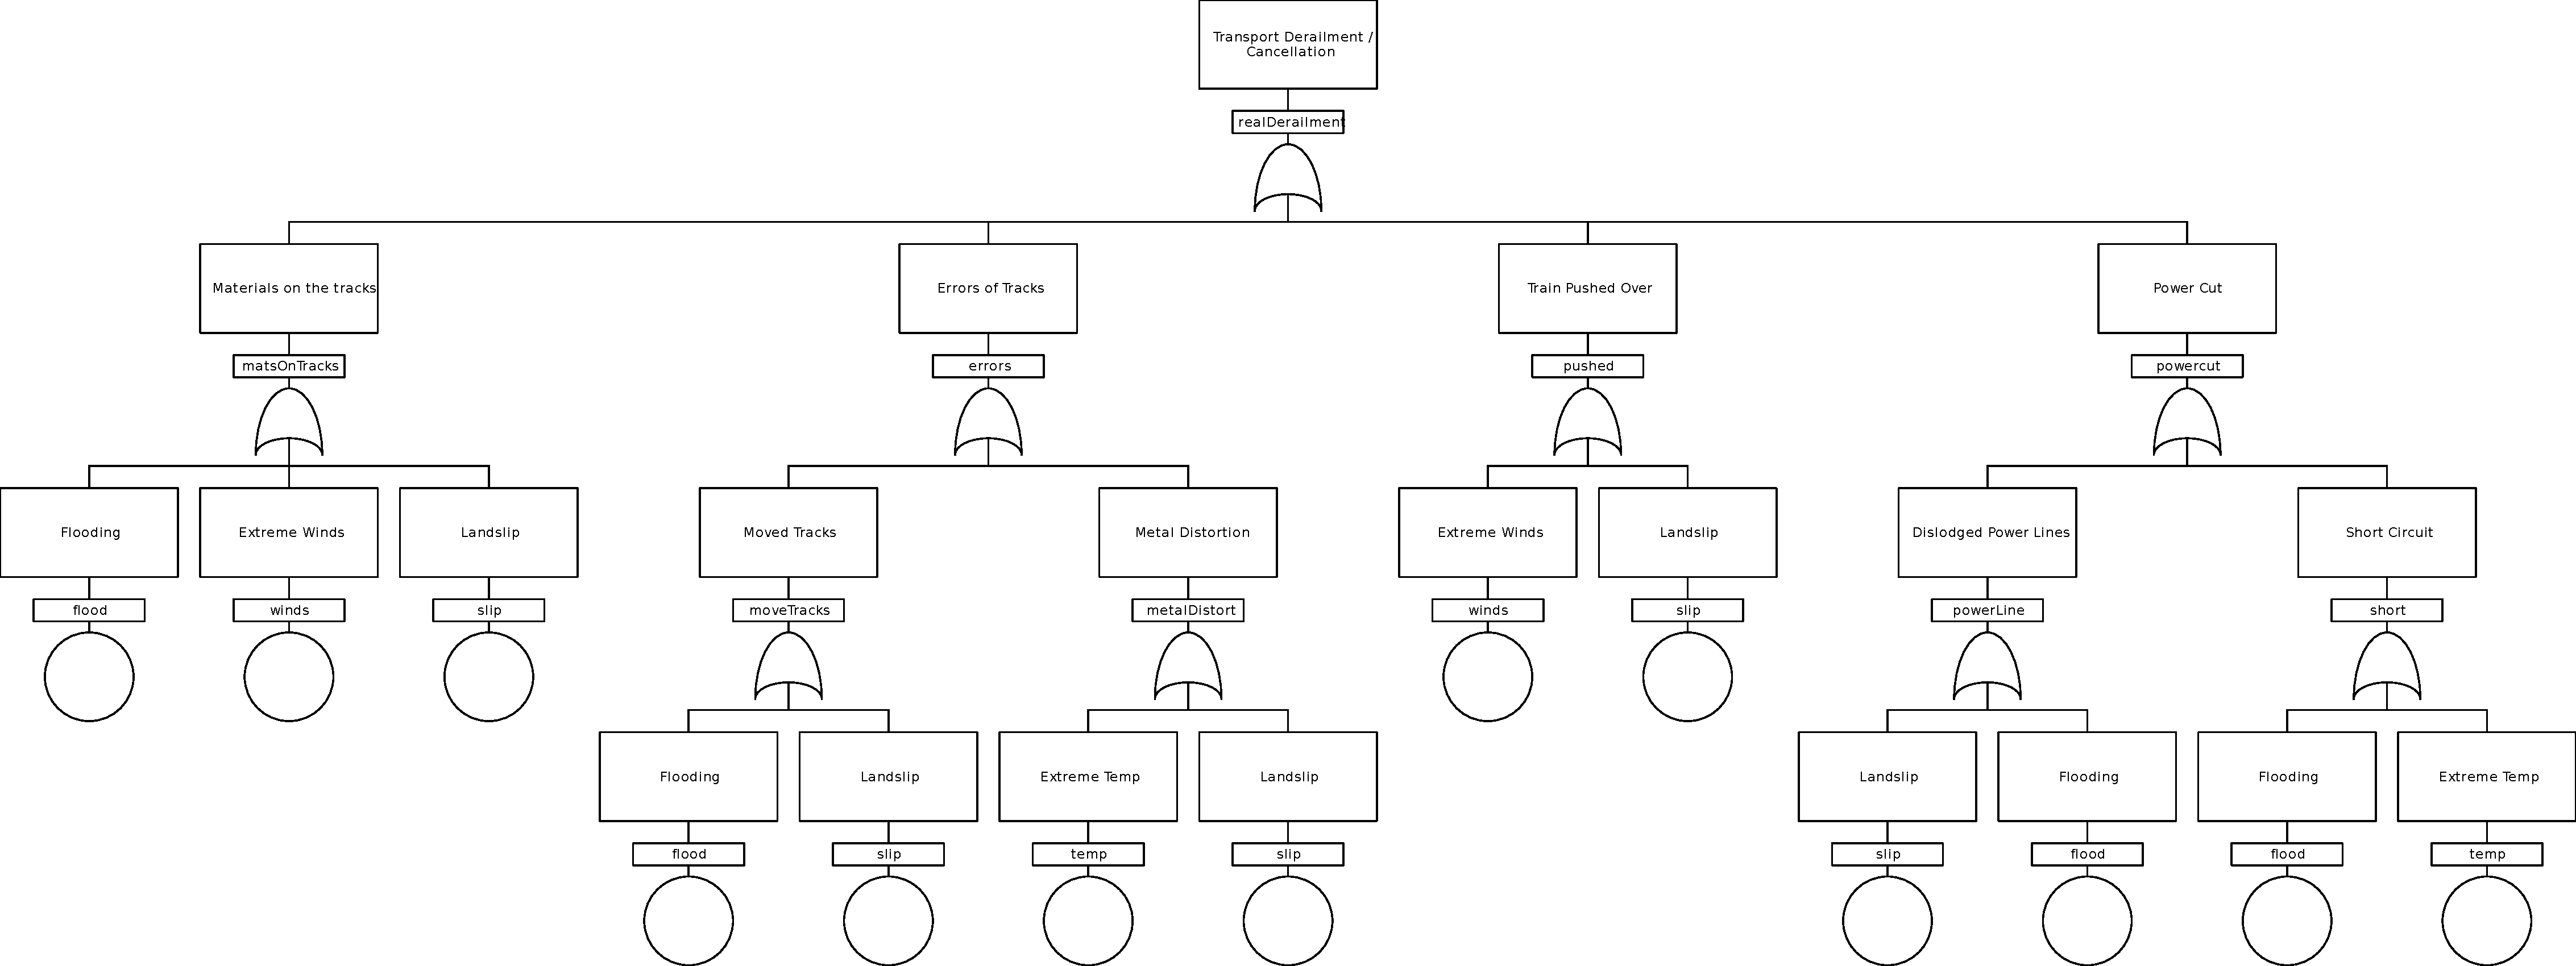
\includegraphics[width=0.95\textheight]{faulttree.png}
	\end{sideways}
	\caption{The resultant fault tree.}
	\label{fig:tool}
\end{figure}

This fault tree was used to create a spreadsheet to allow a user to input the
probabilities of the basic events to determine if the risk of trail derailment has
changed.
The user would insert values for the probabilities of the basic events, which would cause
the values in the second table to update according to the formulas in the cells.
Said formulas are the unions of the probabilities of the events which constitute the
event.
Table \ref{tab:spread} shows an example of a completed spreadsheet for a scenario for
a period of high rail fall.

\begin{table}[h]
	\centering
	\begin{tabular}{|l|l|}
		\hline
		Basic events & Probabilities \\ \hline
		Flooding & 0.110 \\ \hline
		Extreme Winds & 0.170 \\ \hline
		Land Slip & 0.020 \\ \hline
		Extreme Temperatures & 0.120 \\ \hline
		 &  \\ \hline
		Root & Calculations \\ \hline
		Materials on the rails & 0.276 \\ \hline
		Moved Tracks & 0.128 \\ \hline
		Metal Distortion & 0.138 \\ \hline
		Errors of Tracks & 0.248 \\ \hline
		Train Pushed Over & 0.187 \\ \hline
		Dislodged Power Lines & 0.128 \\ \hline
		Short Circuit & 0.217 \\ \hline
		Power Cut Off & 0.317 \\ \hline
		Total & 0.697 \\ \hline
	\end{tabular}
	\caption{An example of a completed spreadsheet.}
	\label{tab:spread}
\end{table}

\FloatBarrier
\section{Results}
\begin{figure}[h]
	\centering
	\begin{subfigure}[b]{0.7\textwidth}
		\includegraphics[width=\textwidth]{tree_1}
	\end{subfigure}
	\begin{subfigure}[b]{0.7\textwidth}
		\includegraphics[width=\textwidth]{tree_2}
	\end{subfigure}
	\begin{subfigure}[b]{0.3\textwidth}
		\includegraphics[width=\textwidth]{tree_3}
	\end{subfigure}
	\caption{Graphs showing the results of the evaluation survey for the fault tree
		based tool}
	\label{fig:eval}
\end{figure}

\begin{figure}[h]
	\centering
	\begin{subfigure}[b]{0.7\textwidth}
		\includegraphics[width=\textwidth]{fmca_1}
	\end{subfigure}
	\begin{subfigure}[b]{0.7\textwidth}
		\includegraphics[width=\textwidth]{fmca_2}
	\end{subfigure}
	\begin{subfigure}[b]{0.3\textwidth}
		\includegraphics[width=\textwidth]{fmca_3}
	\end{subfigure}
	\caption{Graphs showing the results of the evaluation survey for the FMECA
		based tool}
	\label{fig:fmca}
\end{figure}

\FloatBarrier
\section{Evaluation of Tool}
To evaluate the tool, an alternative tool has been created by another group which also
assesses the risk of climate change on the rail network.
The team which created the fault tree based tool consists of Stuart Reilly (2258082R),
Justyna Toporkiewicz (2270645T), Kirsten Edmonstone (2247435E).
The other tool makes use FMECA to create two spread sheets, then compare the values in
each spreadsheet.
The team which created the FMECA based tool consists of Maxwell McLaughlan (2137929M),
Huriyah Hussain (2241433H) and Hannah Fairlie (2204543F).
Figure \ref{fig:eval} shows the results of the evaluation survey for the fault tree based
tool.
Figure \ref{fig:fmca} shows the results of the evaluation survey for the FMECA based tool.
The results for the fault tree based tool are inconsistent as the last graph implies the
system requires a large amount of pre-existing knowledge to make use of, but the third
graph implies the system is easy to use.
Whereas the results for the FMECA based tool all imply the system is easy to make
effective use of.

The people who were selected for the evaluation survey were members of the course.
While these people are better suited then the general public to evaluate the tool, they
are not industry professionals, so the conclusions drawn have limited real world use.

\section{Conclusion}
Overall, the tool produced has limited use.
It is extremely restricted on which basic events it takes into account, and assumes the
only issue the rail network faces is possible train derailment.
The people surveyed are not industry professionals, so the evaluation of their opinions
have limited use.
Therefore, to make the tool useful, a collection of industry professionals should be
surveyed for their opinions on the tool.
The likely outcome of such a survey would be more basic events and possibly more trees
to include more major issues for the rail network.

\end{document}
